
\chapter{$\beta$-Ensembles}

%%%%%%%%%%%%%%%%%%%%%%%%%%%%%%%%%%%%%%%%%%%%%%%%%%%%%%%%%%%%%%%%%%%%%%%%%%%%%%%%%%%%%%%%%%
%%%%%%%%%%%%%%%%%%%%%%%%%%%%%%%%%%%%%%%%%%%%%%%%%%%%%%%%%%%%%%%%%%%%%%%%%%%%%%%%%%%%%%%%%%
\section{Introduction}

In this chapter, we will talk about the Hermite $\beta$-ensembles more in depth. The beta ensembles have wide applications in statistical physics, eningeering, and many other places. They are defined by the joint density of their eigenvalues, and have a special characterization discussed in the next subsection.

%%%%%%%%%%%%%%%%%%%%%%%%%%%%%%%%%%%%%%%%%%%%%%%%%%%%%%%%%%%%%%%%%%%%%%%%%%%%%%%%%%%%%%%%%%

\subsection{Hermite $\beta$-Ensembles}

The Hermite $\beta$-ensembles, also called the Gaussian ensembles, are an important class of random matrix ensembles studied in engineering, statistical physics, and probability theory. Parameterized by $\beta \in \N$ through the Dyson index, this ensemble is charecterized by a few things.

\begin{itemize}
  \item The Dyson index $\beta$ corrosponds to the number of real number of components the subject matrices have.
  \item The subject matrices are classically defined for $\beta = 1,2,4$ and they corrospond to matrices with real, complex, and quaternionic entries. The corrosponding fields are $\R$, $\Cc$, and $\mathbb{H}$.
  \item The matrices in this ensemble, most importantly, have a feature called conjugation invariance. With respect to the conjugation by the respective group of matrices.
  \item Most importantly, the eigenvalues are determined by the joint probability density function given below.
\end{itemize}

\begin{definition}[Hermite $\beta$-ensembles]
The Hermite $\beta$-ensembles, commonly known as the Gaussian ensembles, are an ensemble of random matrices parameterized by $\beta$, and their eigenvalues have the joint probability density function:
\begin{align*}
f_\beta(\Lambda) = c_H^\beta \prod_{i < j} |\lambda_i - \lambda_j|^\beta e^{-1/2\sum_i \lambda_i^2}
\end{align*}
where the normalization constant $c_H^\beta$ is given by:
\begin{align*}
c_H^\beta = (2\pi)^{-n/2} \prod_{j = 1}^n \frac{\Gamma(1 + \beta/2)}{\Gamma(1 + \beta j/2)}
\end{align*}
\end{definition}

To simulate matrices from the $\beta$-ensemble, we will be using a recent result published in ``Matrix Models for Beta Ensembles'' \cite{dimitriu:2018}. This makes the $\beta$-ensemble a canonical example of an implicity distributed matrix; we do not care about the actual distribution of the entries, but rather the effect they have on the eigenvalues (trace) of the matrices. The algorithm used is directly cited from the results of Dumitriu's paper, and can be found in Algorithms B.1.3.

\begin{code}[Hermite Beta = 2 Ensemble]
Let $\mathcal{D} = \mathcal{H}(\beta = 2)$. We can generate $\Ens \sim \D$, an ensemble of $4 \times 4$ Hermite matrices ($\beta = 2$) of size 10 as such:
\end{code}

\begin{lstlisting}[language=R]
# Using the RMAT package
library(RMAT)
ensemble <- RME_beta(N = 4, beta = 2, size = 10)

# Outputs the following
ensemble

...
[[10]]
          [,1]     [,2]      [,3]       [,4]
[1,] 0.3812855 2.592124 0.0000000  0.0000000
[2,] 2.5921244 1.362211 1.4197438  0.0000000
[3,] 0.0000000 1.419744 0.8220259  0.3917667
[4,] 0.0000000 0.000000 0.3917667 -0.9740052
\end{lstlisting}

%%%%%%%%%%%%%%%%%%%%%%%%%%%%%%%%%%%%%%%%%%%%%%%%%%%%%%%%%%%%%%%%%%%%%%%%%%%%%%%%%%%%%%%%%%

\subsection{Dimitriu's Matrix Model}

To generate Hermite $\beta$ matrices, we consider the result of Dimitriu's paper. We obtain the following algorithm.

\begin{algorithm}[Dimitriu's Beta Matrix] \hfill
  \begin{enumerate}
    \item Fix $N \in \N$.
    \item Start by taking a diagonal of $\Normal(0,2)$ variables.
    \item Set both of the nearest off-diagonals to the row that samples from a $\chi(df = df_i) \where df_i = \beta * i$ for columns going from $i = 1$ to $i = n-1$.
  \end{enumerate}
\end{algorithm}

%%%%%%%%%%%%%%%%%%%%%%%%%%%%%%%%%%%%%%%%%%%%%%%%%%%%%%%%%%%%%%%%%%%%%%%%%%%%%%%%%%%%%%%%%%
%%%%%%%%%%%%%%%%%%%%%%%%%%%%%%%%%%%%%%%%%%%%%%%%%%%%%%%%%%%%%%%%%%%%%%%%%%%%%%%%%%%%%%%%%%

\newpage
\section{Spectra}

We know that $\beta$-matrices must be symmetric. So, their eigenvalues must be real. Any imaginary component we observe is simply computational error, and we may safely ignore it. It is good to see that the error is uniform and small.

\begin{remark}[Implicit Distribution]
Note that the beta ensemble is an ensemble characterized by some joint density function on its eigenvalues. So, this is a specific instance of an implcitly distributed matrix. There are many things to consider about $\textbf{identifiability}$ that are subtle, but important. Recall that in our formalization of a specturm as a formal statistic, we vectorized the matrix then tooks the determinant of the characteristic polynomial that came about it. For this reason, we can see that while Dimitriu's model provides an explicit formula, there is an issue of identifiability. That is, given some eigenvalues, there is no injective function to the characteristic polynomial that produced it. Rather, there are infinitly many equivalence classes of characteristic polynomials (and such, random matrices) that surjectively produce a given multiset of eigenvalues.
\end{remark}

\begin{remark}[Floating Point Errors]
Because the model involves diving by $\sqrt{2}$, floating point errors and algorithmic systemic error will yield small, but negligible imaginary components.
\end{remark}

%%%%%%%%%%%%%%%%%%%%%%%%%%%%%%%%%%%%%%%%%%%%%%%%%%%%%%%%%%%%%%%%%%%%%%%%%%%%%%%%%%%%%%%%%%
%%%%%%%%%%%%%%%%%%%%%%%%%%%%%%%%%%%%%%%%%%%%%%%%%%%%%%%%%%%%%%%%%%%%%%%%%%%%%%%%%%%%%%%%%%

\newpage
\section{Dispersions}

Consider the following plot of the sign-sorted eigenvalue dispersions below.

\begin{figure}[h]
	% the options are h = here, t = top, b = bottom, p = page of figures.
	% you can add an exclamation mark to make it try harder, and multiple
	% options if you have an order of preference, e.g.
	% \begin{figure}[h!tbp]
	   
	       \centering
	    % DO NOT ADD A FILENAME EXTENSION TO THE GRAPHIC FILE
	    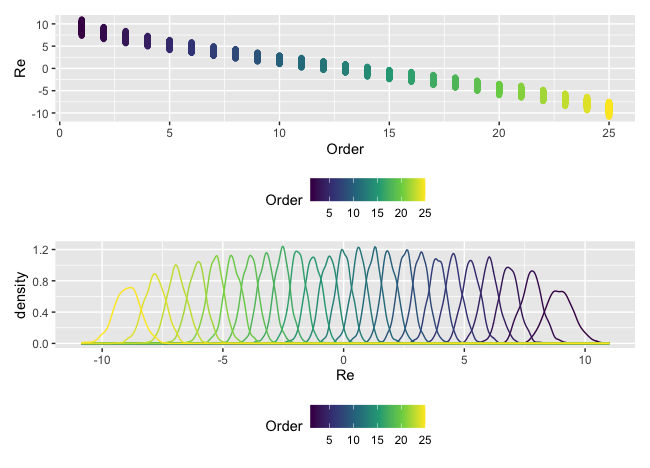
\includegraphics[scale = 0.6]{chapters/graphics/c2_order_sign}
	     \caption{Dispersions of a $\beta = 4$ matrix with respect to ranking difference}
	 \label{subd}
	\end{figure}


